\documentclass[fleqn]{article}

%%%%%%%%%%%%%%%%%%%%% Pre-document %%%%%%%%%%%%%%%%%%%%%
\usepackage{fancyhdr}
\usepackage{titlesec}
\usepackage{float}
\usepackage{array}
\usepackage{nicematrix}
\usepackage{multicol}
\usepackage{enumitem}
\usepackage{listings}
\usepackage{xcolor}
\usepackage{scrextend}

\setlength{\parindent}{0pt} % Remove auto paragraph indents
\renewcommand\labelitemi{{\boldmath$\cdot$}}
\setlength{\mathindent}{0pt}  

% Get rid of those big margins
\usepackage[margin=1in]{geometry}
\newlength\titleindent
\setlength\titleindent{2cm}

\begin{document}

\pagestyle{fancy}
% Header
\fancyhead{}
\fancyhead[L]{Liam Gilligan, Stephanie L'Heureux}
\fancyhead[R]{\thepage}
% No page numbers for footer
\fancyfoot{}

\begin{center}
    \Large{\textbf{Arduino Lab 2}}\\
\end{center}
\vspace{0.25in}

\section{Introduction}
This report discusses the setup, challenges encountered, and solutions implemented in completing the First Arduino Lab. The lab was successful, meeting the specifications by controlling seven LEDs which represented the least significant bits of each ASCII representation of a letter in string, with the sequence advancing to the next letter upon a button press.
\section{Setup}
\subsection{Required components}
\begin{itemize}
    \item[(1)] Solderless breadboard
    \item[(1)] Pushbutton
    \item[(7)] LEDs
    \item[(8)] Resistors
    \item[(15)] Wires
    \item[(1)] USB A/B Cable
    \item[(1)] Arduino Uno
\end{itemize}
\subsection{Pre-lab exercises}
The setup included the completion of two preliminary exercises: one involving blinking an LED, and the other controlling the LED using a push button to ensure familiarity with the Arduino and components. Given the lab group’s strong background in hardware interfacing, the exercises were completed with ease but provided a welcomed refresher on Arduino basics. 
\subsection{Lab setup}
The setup for the primary lab consisted of identifying all the required components and assembling the circuit. During the assembly, a minor issue was encountered in which where the cathode and anode legs of a few LEDs were reversed, causing some LEDs to remain off. This was quickly identified by setting all the LEDs to high on setup to confirm their functionality. Additionally, a multimeter was used to verify that the circuit was fully connected and performing as expected.

\section{Challenges}
Overall, the lab went smoothly, with only minor syntactical and logical errors. These issues were resolved, often by making use of the serial monitor to observe and debug the program's behavior.

The most noteworthy issue occurred after the lab itself was completed, during the process of preparing the .ino file for submission. While renaming the file, it was mistakenly overwritten. As this action was performed on a Linux system from the terminal, there was no trivial way to revert the action and recover the lost content (easily). 
\section{Solutions}

It was concluded attempting to restore the overwritten file content on the Linux system would be a dead end. Therefore, attention was focused on extracting the code from the Arduino. However, this approach was also unsuccessful, as the source code is not stored on the device, only the binary. After evaluating the possibility of using a decompiler and reverse-engineering the original program, it was concluded that the process would be more trouble than it was worth. As a result, a new version of the code was written.
\section{Conclusion}
    % \begin{figure}[H]
    %     \centering
    %     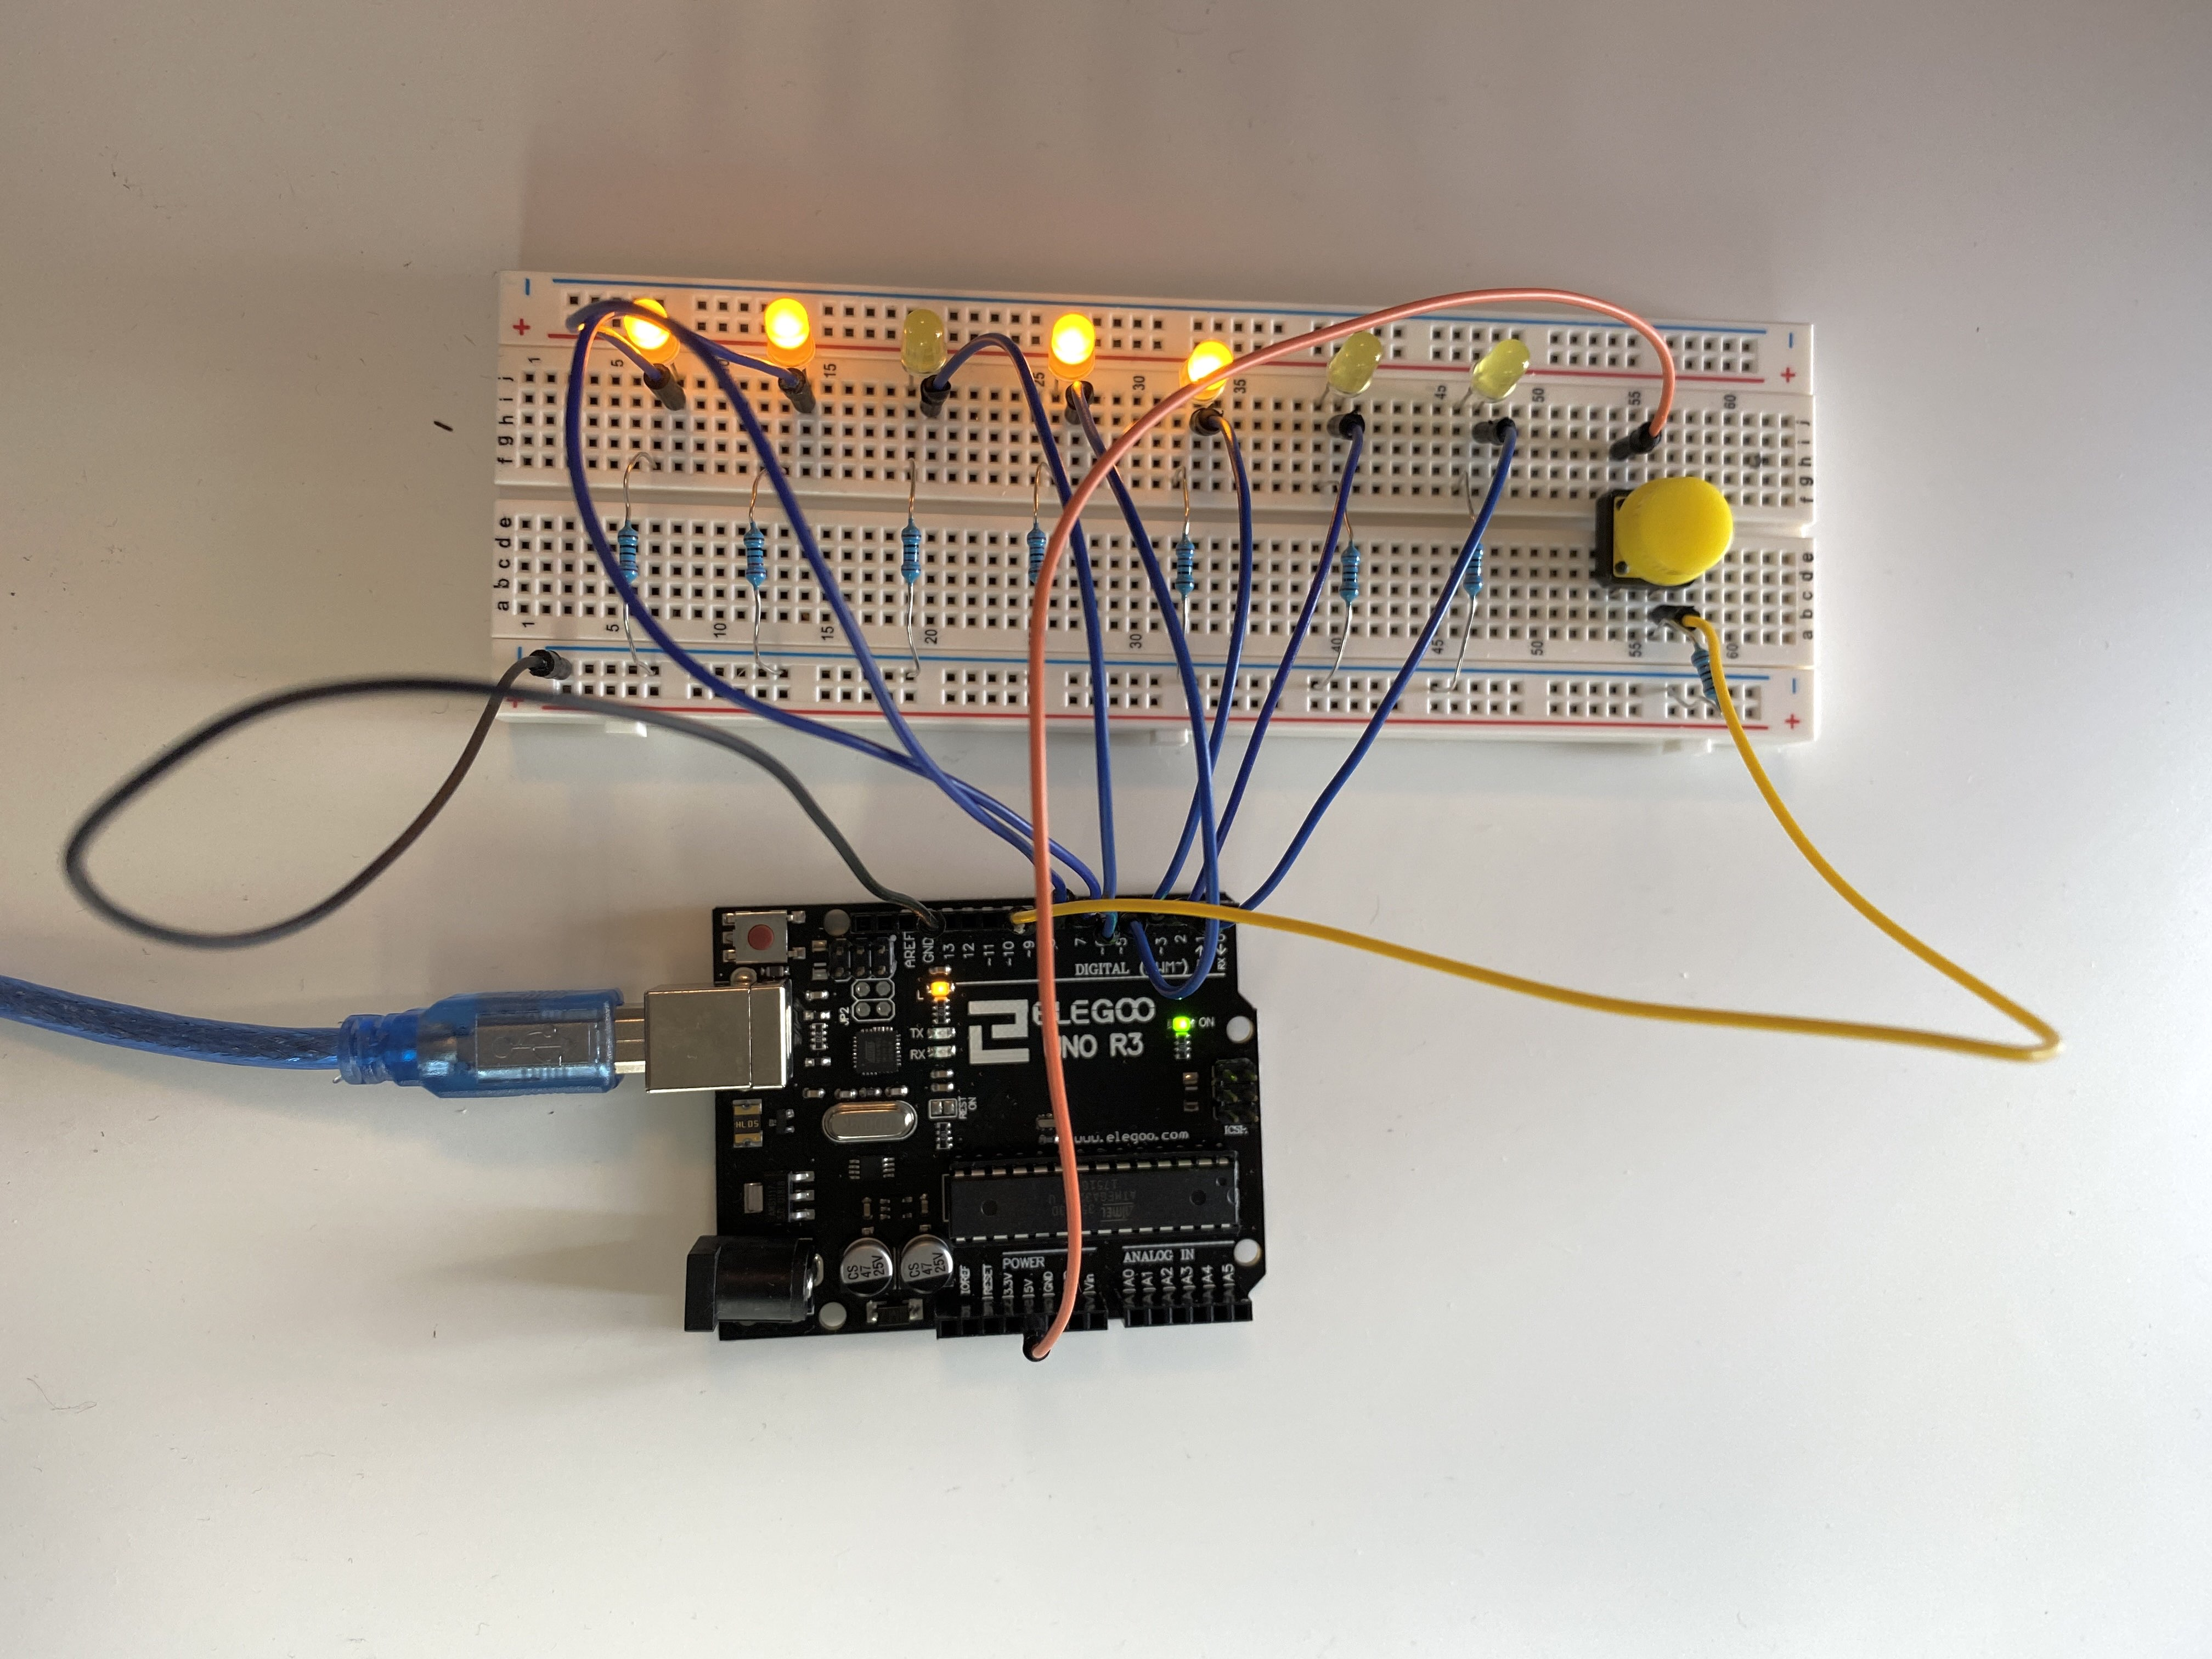
\includegraphics[width=6in]{image.jpg}
    %     \caption{Completed lab with some LEDs illuminated and some dark.}
    % \end{figure}
    Overall, the lab was successful. We developed a program that could be configured to display the names of an (imaginary) user(s) in lights. The wiring was straightforward and well-organized on a breadboard. Additionally, the Arduino serial monitor proved to greatly assist in the debugging process. Following the incident of accidentally overwriting the source code, the importance of using Git for version control was emphasized.
\end{document}
